\label{app:experiments}

This appendix collects three supporting experiments referenced in \Cref{sec:experiments}. All three are run at the full parameter sweep (Experiment~3 with $48{,}000$ raw rows, Experiment~A with $72{,}000$, and Experiment~B with $14{,}400$). These experiments test whether the corrected allocation logic extends beyond the scalar Gaussian DGP and show where the adaptive estimator's safety fallback engages.

% --- Figures moved verbatim from the main paper to fit the 9-page limit ---

\begin{figure}[!h]
  \centering
  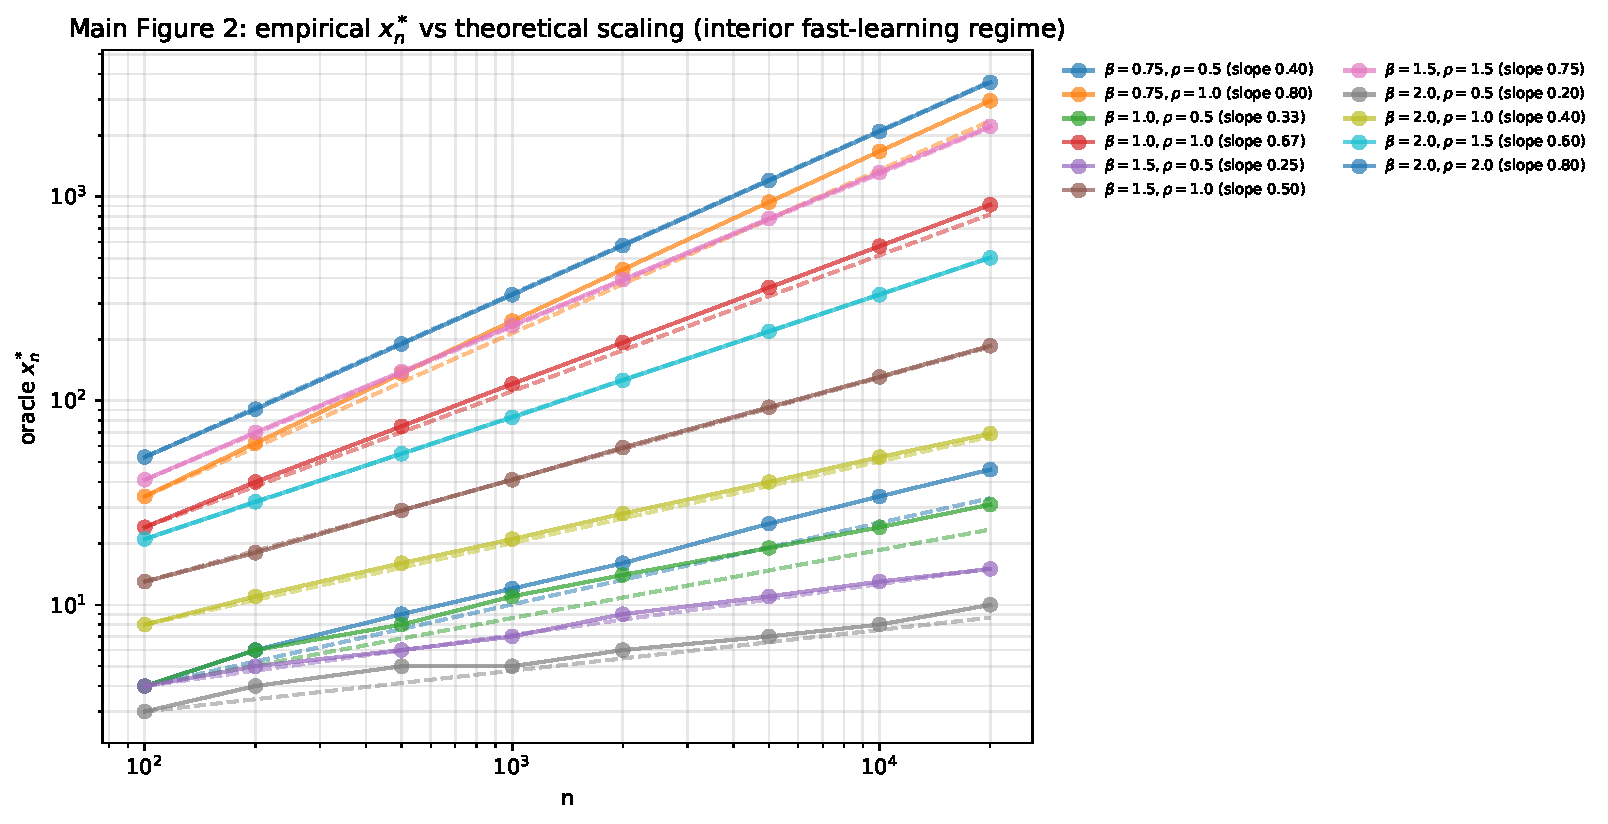
\includegraphics[width=0.95\linewidth]{figures/fig2_scaling_validation.pdf}
  \caption{Empirical and theoretical scaling of the oracle calibration size $\log x_n^\star$ versus $\log n$ for four representative regimes (fixed $m$; slow learner $\beta=0.4,\rho=1$; common fast learner $\beta=1,\rho=1$; boundary $\beta=1,\rho=2$). Solid lines are theoretical slopes from Theorem~\ref{thm:phase}; markers are oracle solutions to the corrected first-order condition on the simulation grid.}
  \label{fig:scaling}
\end{figure}

\begin{figure}[!h]
  \centering
  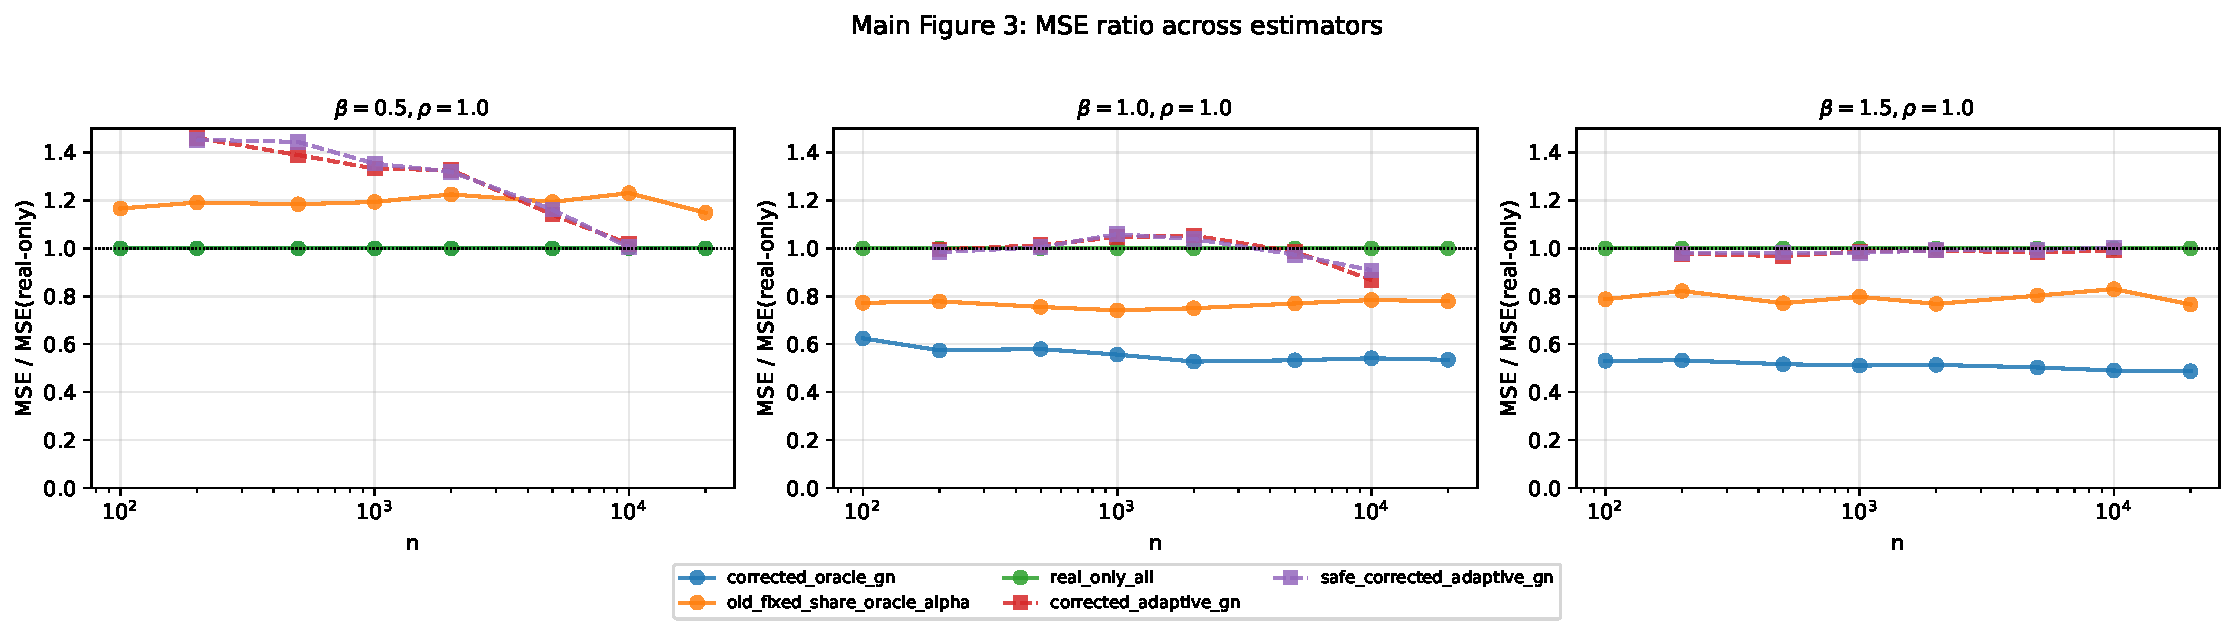
\includegraphics[width=0.95\linewidth]{figures/fig3_mse_comparison.pdf}
  \caption{MSE ratio to \texttt{real\_only\_all} across $n$ for the corrected oracle, the safe corrected oracle (with the safety check from \cref{prop:safe}), naive pooling, the equal-split baseline, the rejected old fixed-share rule, and synthetic-only with full calibration. The corrected oracle is the lower envelope across the entire grid; the old fixed-share rule pays a constant-factor penalty in the fast-learning regime by over-calibrating.}
  \label{fig:mse_compare}
\end{figure}

\begin{figure}[!h]
  \centering
  \begin{subfigure}[t]{0.48\linewidth}
    \centering
    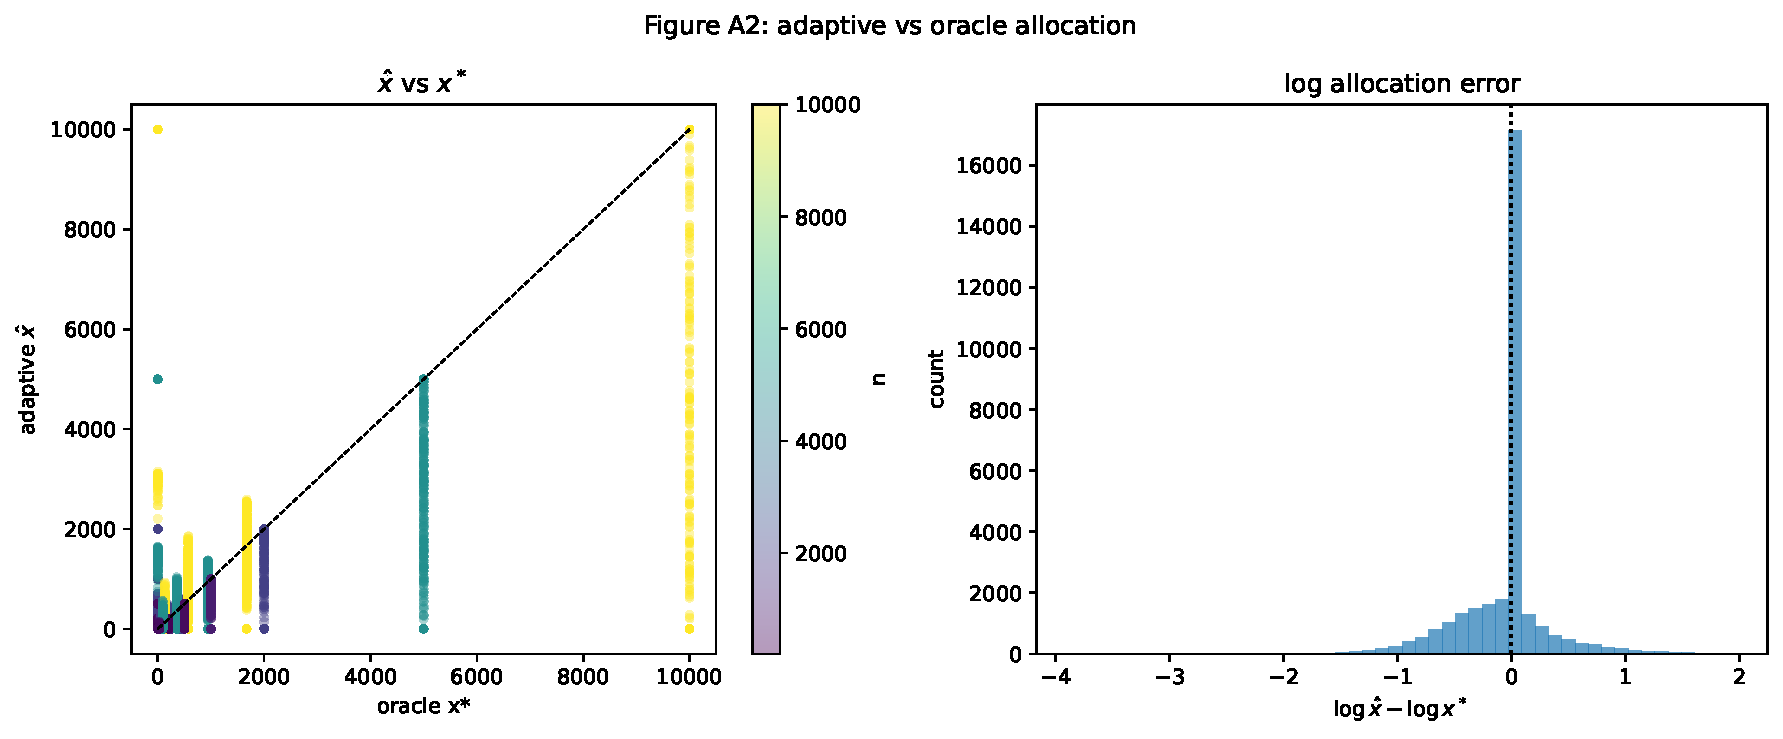
\includegraphics[width=\linewidth]{figures/fig4_adaptive_vs_oracle.pdf}
    \caption{Adaptive allocation.}
    \label{fig:adaptive_alloc}
  \end{subfigure}\hfill
  \begin{subfigure}[t]{0.48\linewidth}
    \centering
    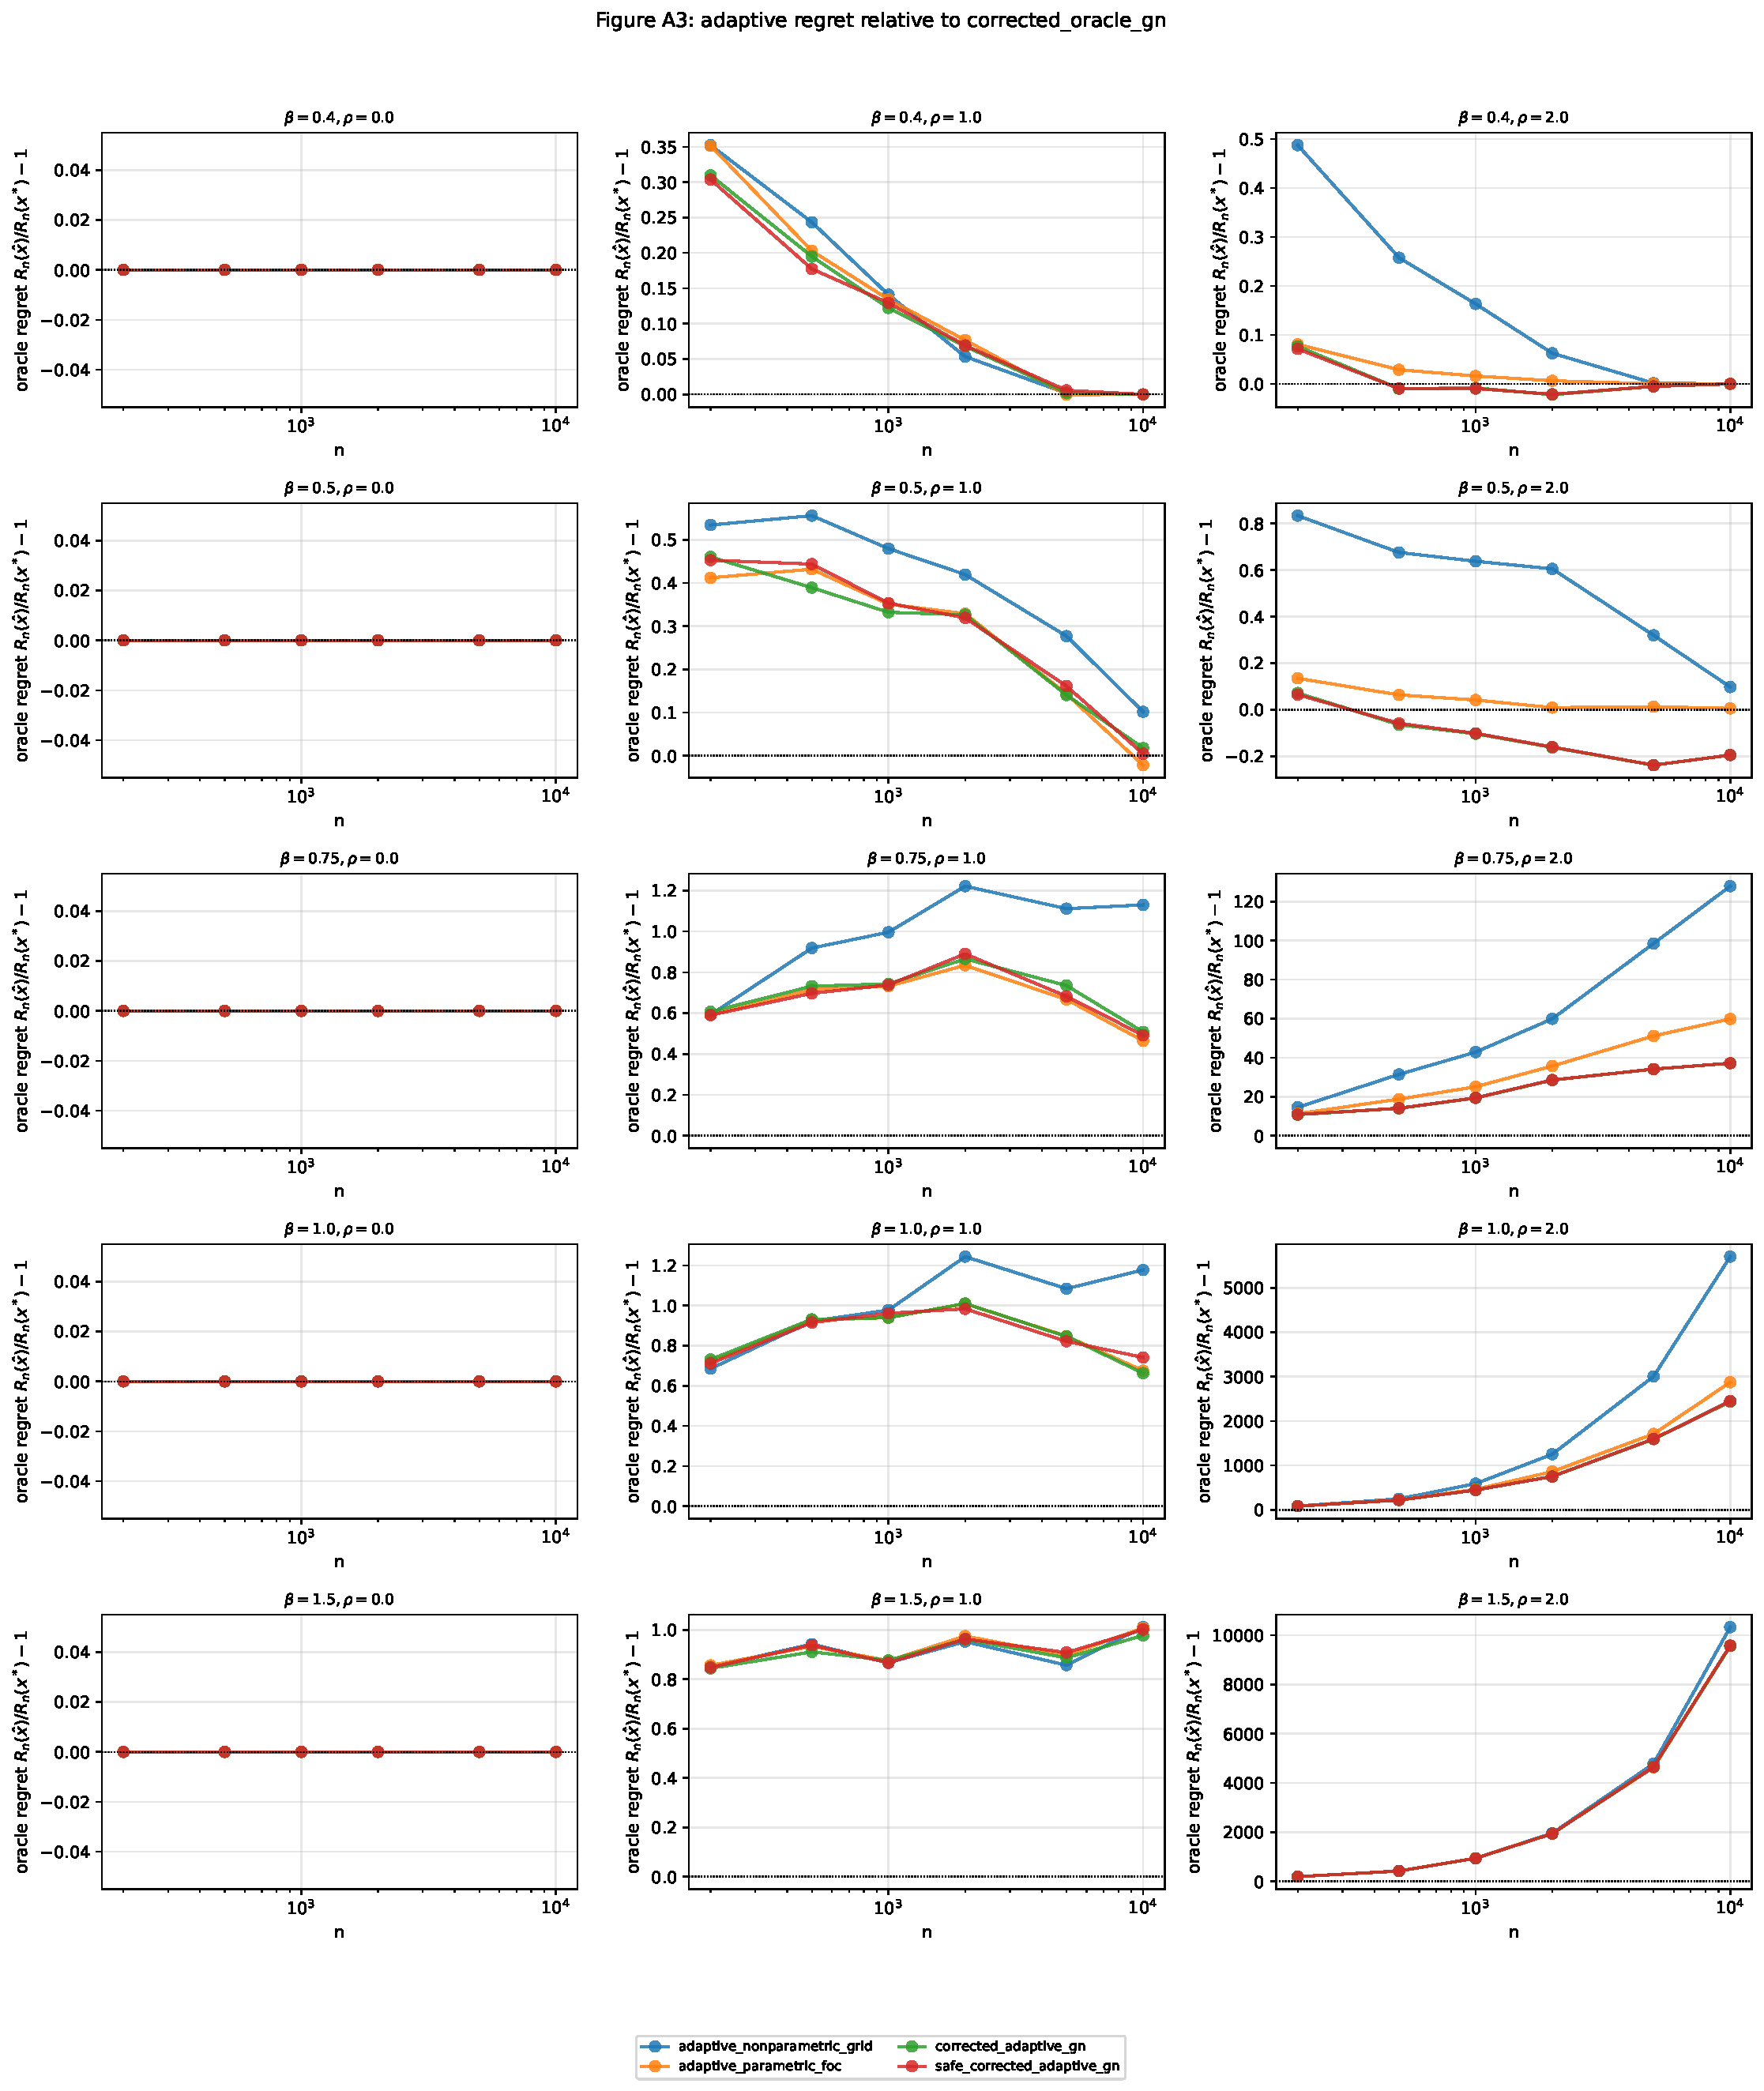
\includegraphics[width=\linewidth]{figures/fig5_adaptive_regret.pdf}
    \caption{Adaptive regret.}
    \label{fig:adaptive_regret}
  \end{subfigure}
  \caption{\emph{Left:} adaptive allocation $\hat x_n$ against oracle $x_n^\circ$ across $(\beta,\rho,n)$ cells. Points along the diagonal indicate close allocation tracking. \emph{Right:} adaptive regret $R_n(\hat x_n)/R_n(x_n^\circ) - 1$ as a function of $n$. The corrected adaptive estimator with safety fallback (Theorem~\ref{thm:adaptive}) usually selects a similar calibration size but still has a visible finite-sample MSE gap at $n \le 10^4$.}
\end{figure}

\begin{figure}[!h]
  \centering
  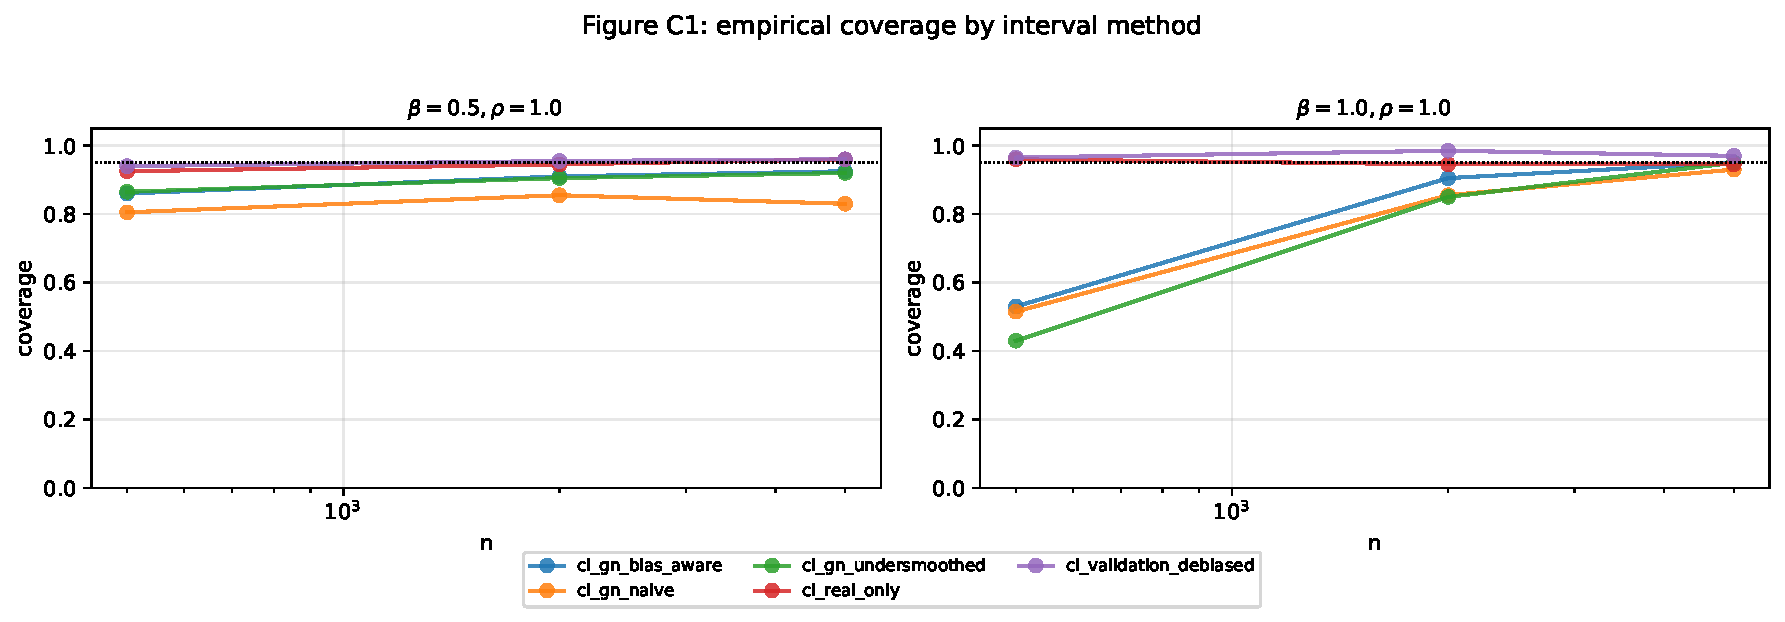
\includegraphics[width=0.95\linewidth]{figures/fig6_coverage.pdf}
  \caption{Empirical coverage of 95\% intervals against $n$ for five interval methods at $\rho=1$ across $\beta\in\{0.4,0.5,0.75,1.0\}$. Dashed line at nominal $0.95$. Naive Wald around the MSE-optimal estimator (\texttt{ci\_gn\_naive}) undercovers when synthetic bias is non-negligible (naive coverage min $0.855$ vs validation-debiased min $0.938$ across the full Experiment~4 grid). Validation debiasing (\texttt{ci\_validation\_debiased}) and the all-real interval (\texttt{ci\_real\_only}) sit closest to nominal coverage; bias-aware widening and undersmoothing only partially close the gap.}
  \label{fig:coverage}
\end{figure}

\subsection{Complete summaries for main experiments}\label{app:main-exp-details}

\paragraph{Experiment~1 scaling details.} \Cref{tab:scaling} reports the representative scaling slopes behind \Cref{ssec:exp1}. The four upper rows are the cells where empirical slopes exceeded theory; the four lower rows are high-$\beta$ cells where the empirical and theoretical slopes agree closely.

\begin{table}[!t]
  \centering
  \caption{Theoretical vs.\ empirical allocation scaling slopes by
  $(\beta,\rho)$.}
  \label{tab:scaling}
  \begin{threeparttable}
  \begin{tabular}{ccccc}
    \toprule
    $\beta$ & $\rho$ & theory slope & empirical slope & SE \\
    \midrule
    $0.75$ & $0.5$ & $0.400$ & $0.453$ & $0.006$ \\
    $0.75$ & $1.0$ & $0.800$ & $0.842$ & $0.003$ \\
    $1.00$ & $0.5$ & $0.333$ & $0.375$ & $0.011$ \\
    $1.00$ & $1.0$ & $0.667$ & $0.684$ & $0.003$ \\
    \midrule
    $1.50$ & $0.5$ & $0.250$ & $0.250$ & $0.006$ \\
    $1.50$ & $1.0$ & $0.500$ & $0.504$ & $0.002$ \\
    $2.00$ & $0.5$ & $0.200$ & $0.204$ & $0.014$ \\
    $2.00$ & $1.0$ & $0.400$ & $0.404$ & $0.003$ \\
    \bottomrule
  \end{tabular}
  \begin{tablenotes}
    \small
    \item[a] Experiment~1 full profile; slopes estimated by OLS of
    $\log x_n^\star$ on $\log n$ across
    $n\in\{100,\ldots,20{,}000\}$.
  \end{tablenotes}
  \end{threeparttable}
\end{table}

\paragraph{Experiment~2 adaptive details.} \Cref{tab:adaptive} gives the headline adaptive MSE ratios and aggregate harm counts. The table is meant to show finite-sample limitations, not only successes: the adaptive estimator is stable relative to naive synthetic-use baselines, but it is not oracle-equivalent on this grid.

\begin{table}[!t]
  \centering
  \caption{Adaptive estimator MSE ratios at the headline cell ($\beta=1$,
  $\rho=1$, $n=10{,}000$) and aggregate harm statistics across the $60$
  non-trivial cells of the Experiment~2 grid.}
  \label{tab:adaptive}
  \begin{threeparttable}
  \small
  \setlength{\tabcolsep}{3pt}
  \begin{tabular}{lcccc}
    \toprule
    method & headline MSE & headline regret & harm cells & max ratio \\
    \midrule
    \texttt{corrected\_oracle\_gn}             & $0.522$ & $0.000$ & --        & --        \\
    \texttt{corrected\_adaptive\_gn}           & $0.867$ & $0.663$ & $21/60$   & $1.460$   \\
    \texttt{safe\_corrected\_adaptive\_gn}     & $0.908$ & $0.741$ & $22/60$   & $1.453$   \\
    \texttt{adaptive\_parametric\_foc}         & $0.874$ & $0.675$ & $29/60$   & $1.432$   \\
    \texttt{adaptive\_nonparametric\_grid}     & $1.136$ & $1.177$ & $44/60$   & $1.834$   \\
    \bottomrule
  \end{tabular}
  \begin{tablenotes}
    \small
    \item[a] ``Harm'' means MSE ratio to \texttt{real\_only\_all} exceeds one.
    Oracle regret is
    $\mathrm{MSE}/\mathrm{MSE}(\texttt{corrected\_oracle\_gn}) - 1$.
  \end{tablenotes}
  \end{threeparttable}
\end{table}

\paragraph{Experiment~4 coverage details.} \Cref{tab:coverage} reports the full-grid coverage range for each interval method.

\begin{table}[!t]
  \centering
  \caption{Coverage by interval method across the full Experiment~4 grid.}
  \label{tab:coverage}
  \begin{threeparttable}
  \begin{tabular}{lccc}
    \toprule
    interval method & coverage min & coverage median & coverage max \\
    \midrule
    \texttt{ci\_gn\_naive}             & $0.855$ & $0.916$ & $0.955$ \\
    \texttt{ci\_gn\_bias\_aware}       & $0.896$ & $0.930$ & $0.957$ \\
    \texttt{ci\_gn\_undersmoothed}     & $0.913$ & $0.936$ & $0.955$ \\
    \texttt{ci\_real\_only}            & $0.938$ & $0.949$ & $0.956$ \\
    \texttt{ci\_validation\_debiased}  & $0.938$ & $0.953$ & $0.964$ \\
    \bottomrule
  \end{tabular}
  \begin{tablenotes}
    \small
    \item[a] Experiment~4 full profile ($280{,}000$ replications), nominal
    level $95\%$. Min/median/max are taken across all $(\beta,\rho,n)$ cells
    in the grid.
  \end{tablenotes}
  \end{threeparttable}
\end{table}

\subsection{Multichannel allocation (Experiment~3)}\label{app:exp3}

\paragraph{Setup.} Experiment~3 generalises the working model to two calibration channels with effective synthetic error
\[
B_n(x_1, x_2) \;=\; v_n + c_1\, x_1^{-2\beta_1} + c_2\, x_2^{-2\beta_2},
\qquad
V_R(x_1, x_2) \;=\; \frac{a}{n - x_1 - x_2},
\]
so each channel has its own learning exponent and bias-decay constant. Defaults are $a = c_1 = c_2 = \sigma_S^2 = 1$ and $m_n = n$ (so $\rho = 1$), and the learning-exponent pairs are $(\beta_1, \beta_2) \in \{(0.5, 1.0),\ (0.75, 1.5),\ (0.4, 1.0)\}$. Channel~1 plays the role of a slow channel (e.g.\ retrieval conditioning) and channel~2 the role of a fast channel (e.g.\ fine-tuning). The full Experiment~3 sweep produces $48{,}000$ raw replication rows.

\paragraph{KKT verification.} The corrected multichannel oracle equalises the per-channel marginal value at any interior optimum: for every active channel~$k$,
\[
MV_k(\mathbf{x}) \;=\; 2\beta_k\, a\, c_k\, x_k^{-(2\beta_k + 1)}
\;=\; B_n(\mathbf{x})^2,
\]
which is the natural KKT generalisation of the single-channel FOC in \Cref{prop:foc}. Intuitively, at an interior optimum the marginal MSE reduction from spending one more real observation on calibration must be the same in every active channel; otherwise reallocating one observation from a low-$MV$ channel to a high-$MV$ channel would strictly improve risk. The corrected multichannel oracle realises this equality by construction, while the old multichannel fixed-share rule $\lambda_k^{\mathrm{old}} = 2\beta_k / (1 + 2\sum_j \beta_j)$ generally does not. \Cref{fig:multi_surface} plots the two-channel risk surface $R_n(x_1, x_2)$ with each method's selected allocation overlaid, and \Cref{fig:multi_mv} plots $MV_1$ versus $MV_2$ at the selected allocations.

\paragraph{Results.} \Cref{tab:multi_perf} reports the median and maximum MSE ratio of each method to the corrected multichannel oracle across the full grid. The corrected oracle dominates: \texttt{best\_single\_channel\_oracle} sits at median $1.147$, \texttt{equal\_split\_two\_channels} at $1.493$, and \texttt{old\_multichannel\_fixed\_share} at $2.240$. The fixed-share rule's roughly $2\times$ MSE inflation matches the qualitative prediction of Theorem~\ref{thm:phase}: when both channels learn fast and $\rho = 1$, the optimal share in each channel vanishes with $n$, while the fixed-share rule allocates a constant fraction of real data to calibration regardless of $n$. No full-profile cell beats the corrected multichannel oracle in Monte~Carlo MSE.

\begin{table}[!t]
  \centering
  \caption{Multichannel performance summary (Experiment~3, full profile).
  Median and maximum MSE ratio to \texttt{corrected\_multichannel\_oracle}
  across the $(\beta_1, \beta_2, n)$ grid.}
  \label{tab:multi_perf}
  \begin{threeparttable}
  \begin{tabular}{lcc}
    \toprule
    method & median MSE ratio & max MSE ratio \\
    \midrule
    \texttt{corrected\_multichannel\_oracle}    & $1.000$ & $1.000$ \\
    \texttt{best\_single\_channel\_oracle}      & $1.147$ & $1.666$ \\
    \texttt{equal\_split\_two\_channels}        & $1.493$ & $1.745$ \\
    \texttt{old\_multichannel\_fixed\_share}    & $2.240$ & $3.217$ \\
    \bottomrule
  \end{tabular}
  \begin{tablenotes}
    \small
    \item[a] Full profile ($48{,}000$ raw rows) across three
    $(\beta_1, \beta_2)$ pairs and the $n$ grid;
    \texttt{corrected\_multichannel\_oracle} is the per-cell benchmark,
    ratios are aggregated across cells. No cell beats the corrected
    multichannel oracle in Monte~Carlo MSE.
  \end{tablenotes}
  \end{threeparttable}
\end{table}

\subsection{Tabular semi-synthetic benchmark (Experiment~A)}\label{app:expA}

\paragraph{Setup.} Experiment~A tests the adaptive method on the UCI Adult / Census Income tabular dataset using the pseudo-population protocol of \Cref{sec:experiments}: the cleaned full dataset is treated as $\mathcal{D}_{\mathrm{pop}}$, real samples of size $n$ are drawn without replacement, and the ground truth is the pseudo-population value of the estimand. We report two estimands: the binary income outcome mean $\theta_1^\star = \mathbb{E}[Y]$ and the subgroup gap $\theta_2^\star = \mathbb{E}[Y \mid G = 1] - \mathbb{E}[Y \mid G = 0]$. The synthetic generator is the Gaussian-copula baseline (\texttt{gaussian\_copula}, with eigenvalue-clipped correlation matrix to guard against rank-deficient calibration samples). The grid is $n \in \{200, 500, 1000, 2000, 5000\}$ and $m \in \{n, 5n, 10n\}$. The full Experiment~A sweep produces $72{,}000$ raw rows across $45$ retained cells.

\paragraph{Adaptive behaviour.} Across the $45$ retained cells of the tabular grid, both \texttt{corrected\_adaptive\_gn} and \texttt{safe\_corrected\_adaptive\_gn} fall back to the all-real estimator in $45/45$ cells, with median and maximum MSE ratio to \texttt{real\_only\_all} of exactly $1.000$ and zero harmful cells (mean fallback rate $1.000$). \texttt{validation\_debiased\_gn} also returns the all-real point estimate in $45/45$ cells. In contrast, the rejected and naive baselines are uniformly harmful: \texttt{old\_fixed\_share\_plugin\_alpha} sits at median $1.294$ (max $1.501$, harmful in $36/36$ evaluable cells), \texttt{fixed\_half\_split\_plugin\_alpha} at median $3.519$ (max $4.316$, harmful in $45/45$), \texttt{naive\_pooling} at median $5.439$ (max $117.166$, harmful in $45/45$), and \texttt{synthetic\_only\_full\_calibration} at median $8.874$ (max $141.827$, harmful in $45/45$). \Cref{fig:tabular_main} shows the composite view (learning curve plus MSE ratio); \Cref{fig:tabular_learning} isolates the empirical learning curve $\log\widehat{b^2}(x)$ versus $\log x$ on the Adult estimand, and \Cref{fig:tabular_mse} shows the per-method MSE ratio bar plot.

\paragraph{Interpretation.} The full-profile setting does not place the Gaussian-copula generator in a regime where synthetic data helps: the empirical bias curve does not decay rapidly enough at the calibration sizes available within $n \le 5000$ to satisfy the safety margin $\hat x \widehat B_n(\hat x) < \hat a$. The conservative fallback is the desired behavior. Under uncertainty about the learning curve, returning the all-real estimator caps the worst-case loss at zero rather than the order-of-magnitude MSE inflation incurred by naive pooling and synthetic-only baselines (which lack such a fallback). A richer generator family (e.g.\ CTGAN, TVAE, or TabDDPM) may be needed to reach a regime where synthetic data helps, as predicted by Theorem~\ref{thm:phase}; we flag this as future work and report \Cref{tab:tabular_perf} as a lower bound on safety, not an upper bound on adaptive efficacy.

\begin{table}[!t]
  \centering
  \caption{Tabular semi-synthetic performance summary (Experiment~A, full
  profile). Aggregates across the $45$ retained cells of the $n \times m$
  grid for the Adult-pseudo-population mean and subgroup gap.}
  \label{tab:tabular_perf}
  \begin{threeparttable}
  \resizebox{\textwidth}{!}{%
  \begin{tabular}{lccccc}
    \toprule
    method & cells & median MSE ratio & max MSE ratio & harmful cells & mean fallback \\
    \midrule
    \texttt{corrected\_adaptive\_gn}            & $45$ & $1.000$ & $1.000$   & $0/45$  & $1.000$ \\
    \texttt{safe\_corrected\_adaptive\_gn}      & $45$ & $1.000$ & $1.000$   & $0/45$  & $1.000$ \\
    \texttt{validation\_debiased\_gn}           & $45$ & $1.000$ & $1.000$   & $0/45$  & $1.000$ \\
    \texttt{old\_fixed\_share\_plugin\_alpha}   & $36$ & $1.294$ & $1.501$   & $36/36$ & $0.000$ \\
    \texttt{fixed\_half\_split\_plugin\_alpha}  & $45$ & $3.519$ & $4.316$   & $45/45$ & $0.000$ \\
    \texttt{naive\_pooling}                     & $45$ & $5.439$ & $117.166$ & $45/45$ & $0.000$ \\
    \texttt{synthetic\_only\_full\_calibration} & $45$ & $8.874$ & $141.827$ & $45/45$ & $0.000$ \\
    \bottomrule
  \end{tabular}
  }
  \begin{tablenotes}
    \small
    \item[a] Full profile ($72{,}000$ raw rows); UCI Adult dataset;
    \texttt{gaussian\_copula} generator with eigenvalue-clipped correlation
    matrix. ``Harmful'' means MSE ratio to \texttt{real\_only\_all} strictly
    exceeds one. The adaptive variants engage the safe fallback in all $45$
    cells, so their MSE matches \texttt{real\_only\_all} exactly. The
    \texttt{old\_fixed\_share\_plugin\_alpha} row reports $36$ cells because
    the plug-in $\hat\alpha$ is undefined in the $9$ cells where the
    plug-in bias estimate is non-positive.
  \end{tablenotes}
  \end{threeparttable}
\end{table}

\subsection{Causal semi-synthetic benchmark (Experiment~B)}\label{app:expB}

\paragraph{Setup.} Experiment~B targets the average treatment effect $\tau^\star = \mathbb{E}[Y(1) - Y(0)]$ on an IHDP-style semi-synthetic benchmark. The real estimator is augmented inverse-probability-weighting (\texttt{real\_only\_aipw}) with cross-fit nuisance functions; the synthetic generator is the linear outcome model (\texttt{linear\_outcome\_model}). The grid is $n \in \{200, 500, 1000, 2000, 5000\}$ with $m \in \{n, 5n, 10n\}$ across $8$ retained cells. The full Experiment~B sweep produces $14{,}400$ raw rows.

\paragraph{Adaptive behaviour.} The adaptive estimators avoid the large losses seen in naive synthetic-use baselines, but they still show mild residual harm at this profile. \texttt{safe\_corrected\_adaptive\_gn} is harmful in $8/8$ cells with median MSE ratio $1.084$ and maximum $1.181$ (mean fallback $0.811$); \texttt{corrected\_adaptive\_gn} is harmful in $8/8$ cells with median $1.086$ and maximum $1.241$ (mean fallback $0.783$). The remaining baselines are dominated: \texttt{synthetic\_only\_full\_calibration} sits at median $1.276$ (max $1.642$, harmful in $8/8$); \texttt{validation\_debiased\_gn} at median $1.459$ (max $1.889$, harmful in $8/8$, fallback $0.770$); \texttt{naive\_pooling} at median $1.679$ (max $2.122$, harmful in $8/8$); \texttt{old\_fixed\_share\_plugin\_alpha} at median $1.760$ (max $2.264$, harmful in $8/8$); \texttt{fixed\_half\_split\_plugin\_alpha} at median $2.277$ (max $4.075$, harmful in $8/8$); and the \texttt{real\_only\_diff\_in\_means} non-AIPW baseline at median $5.415$ (max $15.472$). \texttt{real\_only\_aipw} is the per-cell benchmark at ratio $1.000$ by construction. \Cref{fig:causal_learning} plots the empirical ATE-bias learning curve and \Cref{fig:causal_mse} the per-method MSE ratio.

\paragraph{Interpretation.} ATE-bias learning is intrinsically harder than mean-bias learning because the held-out validation estimator $\hat b_V(x) = \hat\tau_S(x) - \hat\tau_R^V$ inherits the variance of two nuisance-function estimates, which inflates $\widehat{b^2}(x)$ at small calibration sizes and pushes the safety margin toward fallback before the true bias has actually decayed. The $1.086$ median ratio for \texttt{corrected\_adaptive\_gn} indicates that the method remains relatively stable and outperforms every other synthetic-augmentation baseline in this benchmark, but it is not yet beneficial against the AIPW real-only benchmark; we treat this as a calibration-sample-size limitation of the IHDP-style benchmark, not a contradiction of Theorem~\ref{thm:adaptive}.

\begin{table}[!t]
  \centering
  \caption{Causal semi-synthetic performance summary (Experiment~B, full
  profile). Aggregates across the $8$ retained cells of the $n \times m$ grid
  for IHDP-style ATE.}
  \label{tab:causal_perf}
  \begin{threeparttable}
  \resizebox{\textwidth}{!}{%
  \begin{tabular}{lccccc}
    \toprule
    method & cells & median MSE ratio & max MSE ratio & harmful cells & mean fallback \\
    \midrule
    \texttt{safe\_corrected\_adaptive\_gn}      & $8$ & $1.084$ & $1.181$  & $8/8$ & $0.811$ \\
    \texttt{corrected\_adaptive\_gn}            & $8$ & $1.086$ & $1.241$  & $8/8$ & $0.783$ \\
    \texttt{synthetic\_only\_full\_calibration} & $8$ & $1.276$ & $1.642$  & $8/8$ & $0.000$ \\
    \texttt{validation\_debiased\_gn}           & $8$ & $1.459$ & $1.889$  & $8/8$ & $0.770$ \\
    \texttt{naive\_pooling}                     & $8$ & $1.679$ & $2.122$  & $8/8$ & $0.000$ \\
    \texttt{old\_fixed\_share\_plugin\_alpha}   & $8$ & $1.760$ & $2.264$  & $8/8$ & $0.000$ \\
    \texttt{fixed\_half\_split\_plugin\_alpha}  & $8$ & $2.277$ & $4.075$  & $8/8$ & $0.000$ \\
    \texttt{real\_only\_diff\_in\_means}        & $8$ & $5.415$ & $15.472$ & $8/8$ & $0.000$ \\
    \bottomrule
  \end{tabular}
  }
  \begin{tablenotes}
    \small
    \item[a] Full profile ($14{,}400$ raw rows); IHDP-style ATE;
    \texttt{linear\_outcome\_model} generator; AIPW real estimator with
    cross-fit nuisance functions. ``Harmful'' means MSE ratio to
    \texttt{real\_only\_aipw} strictly exceeds one.
    \texttt{real\_only\_aipw} is the benchmark at ratio one by construction.
  \end{tablenotes}
  \end{threeparttable}
\end{table}


% Figures referenced from appendix C/D/E
\begin{figure}[!t]
  \centering
  \begin{subfigure}[t]{0.48\linewidth}
    \centering
    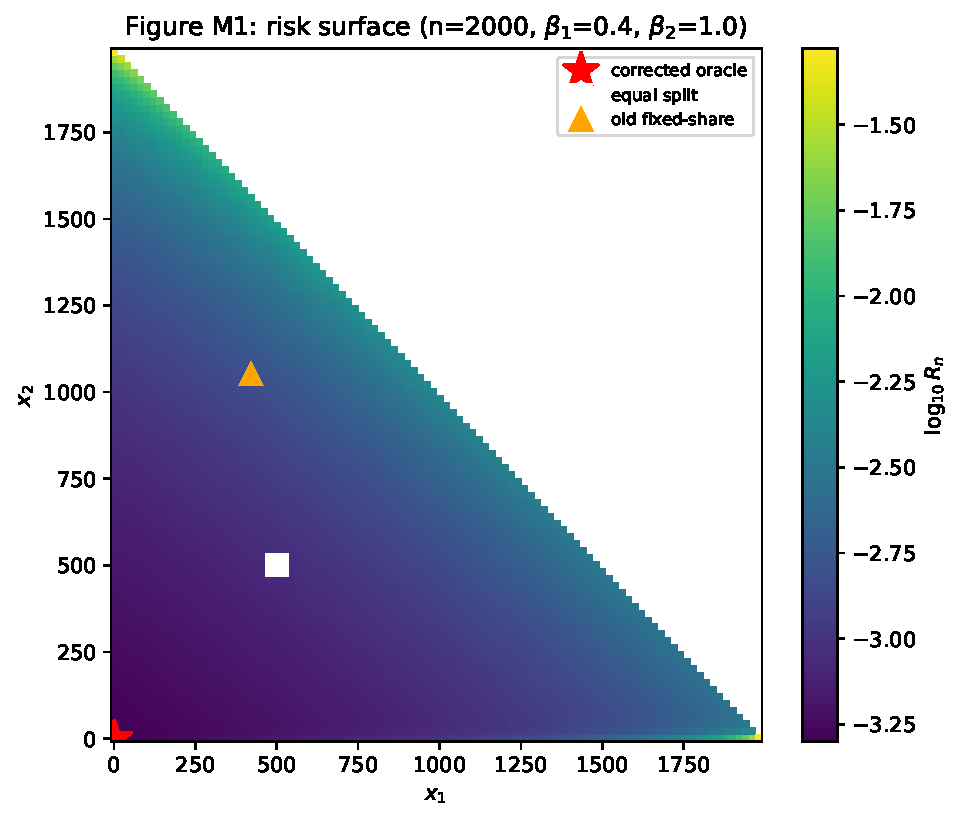
\includegraphics[width=\linewidth]{figures/figM1_risk_surface.pdf}
    \caption{Risk surface.}
    \label{fig:multi_surface}
  \end{subfigure}\hfill
  \begin{subfigure}[t]{0.48\linewidth}
    \centering
    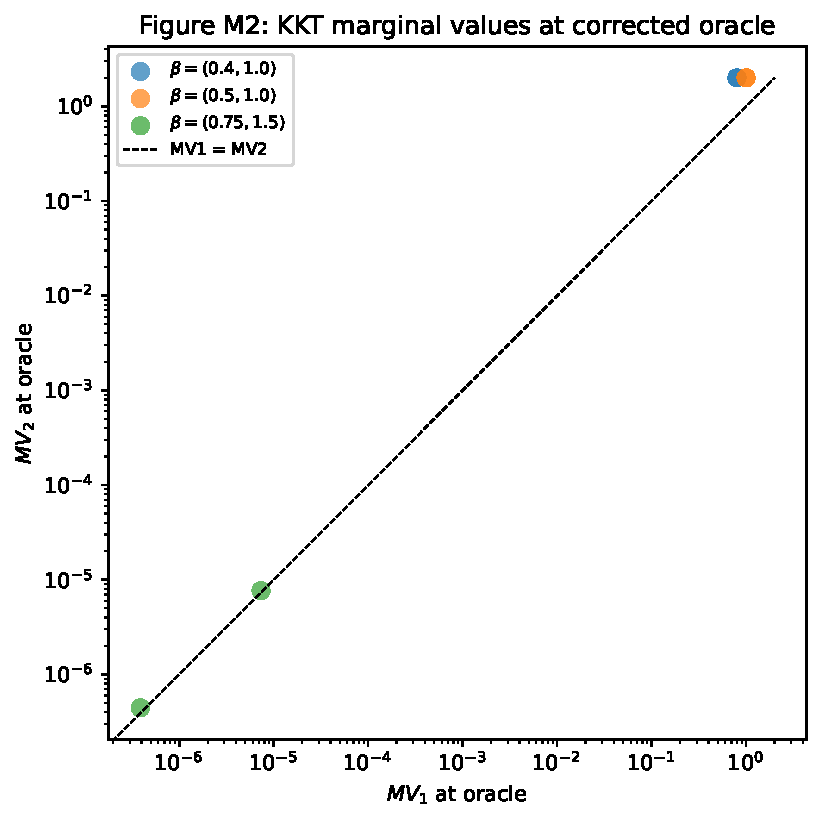
\includegraphics[width=\linewidth]{figures/figM2_marginal_values.pdf}
    \caption{Marginal values.}
    \label{fig:multi_mv}
  \end{subfigure}
  \caption{\emph{Left:} two-channel risk surface $R_n(x_1,x_2)$ over the feasible triangle for representative $(\beta_1,\beta_2)=(0.5,1.0)$, $n=2000$. Markers indicate corrected oracle, equal split, old fixed-share, and best single-channel allocations. \emph{Right:} marginal-value diagnostic: the corrected oracle equalizes per-channel marginal MSE reduction across active channels.}
\end{figure}

\begin{figure}[!t]
  \centering
  \begin{subfigure}[t]{0.48\linewidth}
    \centering
    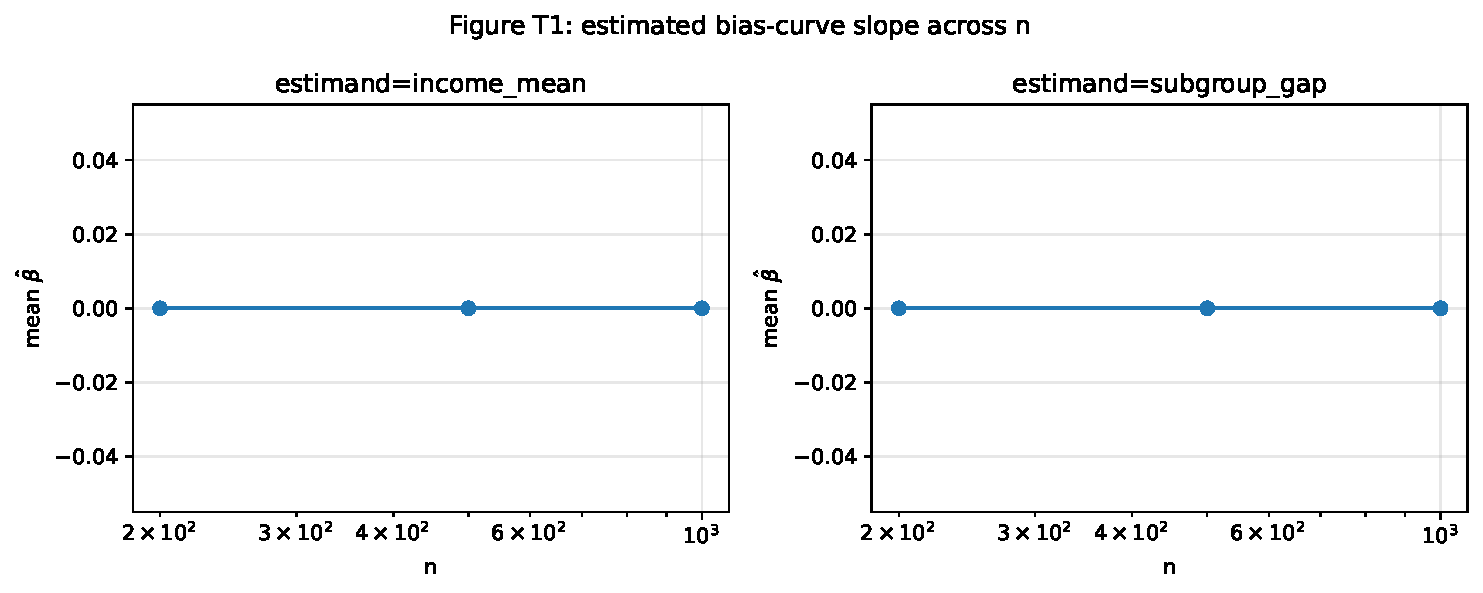
\includegraphics[width=\linewidth]{figures/figT1_tabular_learning.pdf}
    \caption{Learning curve.}
    \label{fig:tabular_learning}
  \end{subfigure}\hfill
  \begin{subfigure}[t]{0.48\linewidth}
    \centering
    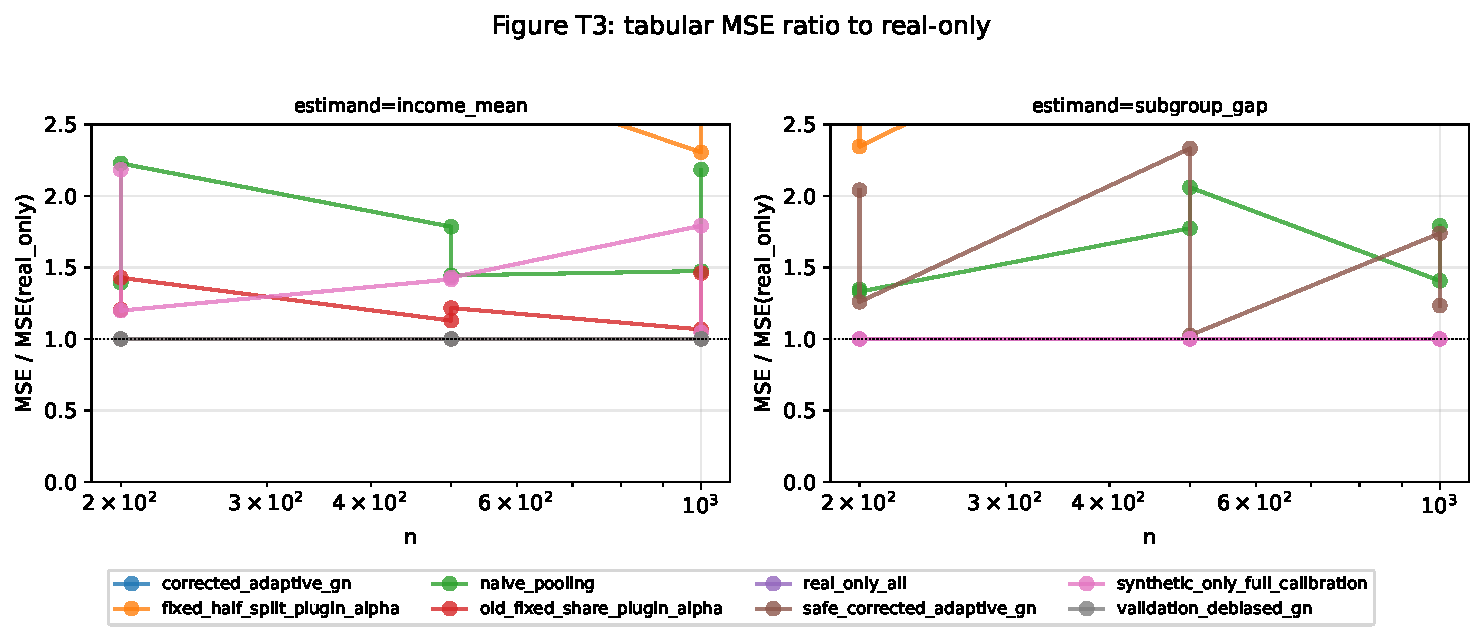
\includegraphics[width=\linewidth]{figures/figT3_tabular_mse.pdf}
    \caption{MSE ratios.}
    \label{fig:tabular_mse}
  \end{subfigure}
  \caption{\emph{Left:} pilot learning curve $\log\widehat{b^2}(x)$ versus $\log x$ for the Adult tabular benchmark with the bootstrap-smoothed generator. \emph{Right:} per-method MSE ratio to real-only across $n$. The corrected adaptive method falls back to all-real in this full-profile setting, while naive pooling and synthetic-only are uniformly harmful.}
\end{figure}

\begin{figure}[!t]
  \centering
  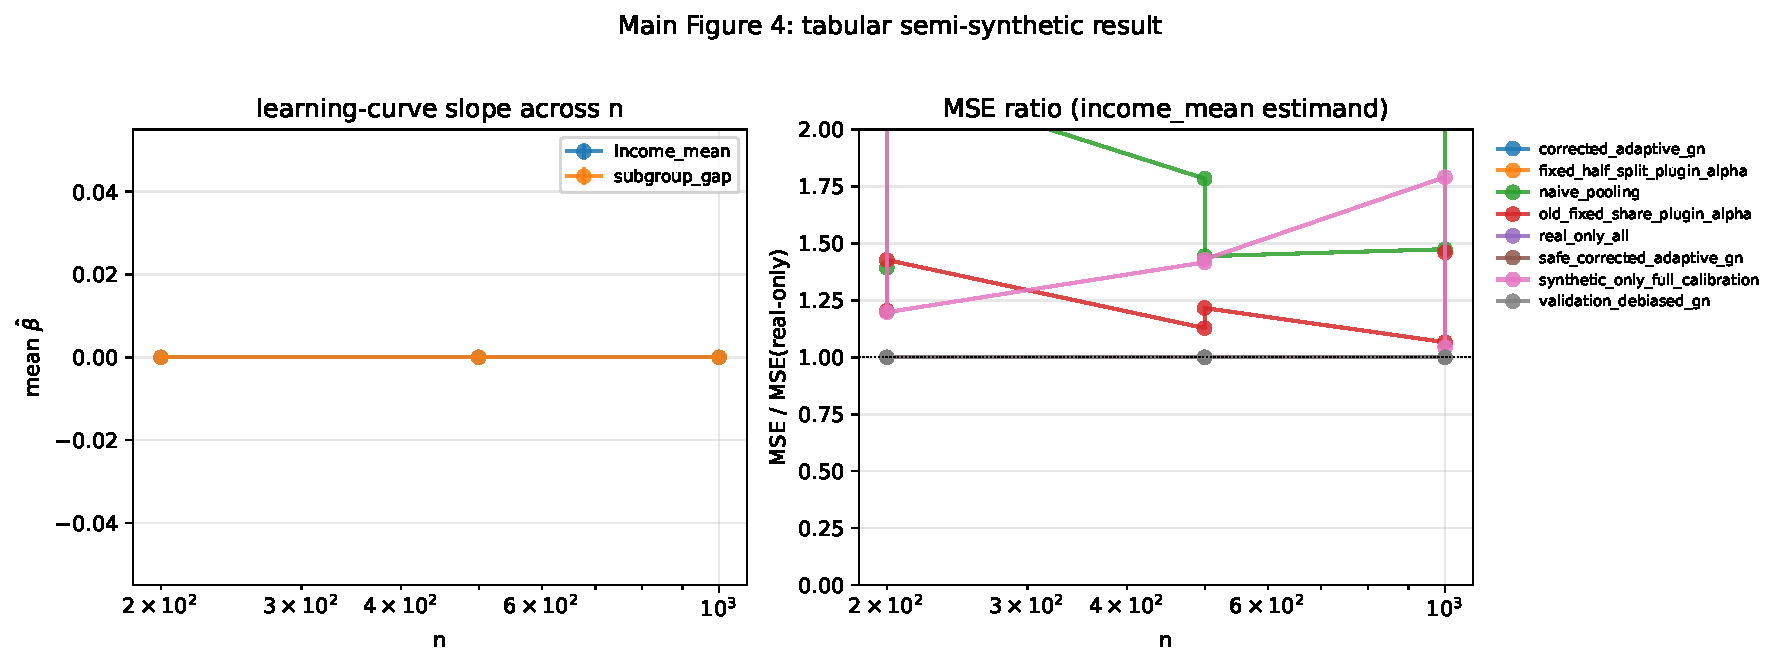
\includegraphics[width=0.85\linewidth]{figures/figT_semisynth.pdf}
  \caption{Tabular semi-synthetic composite (Adult, bootstrap-smoothed generator, full profile): empirical learning curve and MSE ratio summary; mirrors \cref{fig:tabular_learning,fig:tabular_mse}.}
  \label{fig:tabular_main}
\end{figure}

\begin{figure}[!t]
  \centering
  \begin{subfigure}[t]{0.48\linewidth}
    \centering
    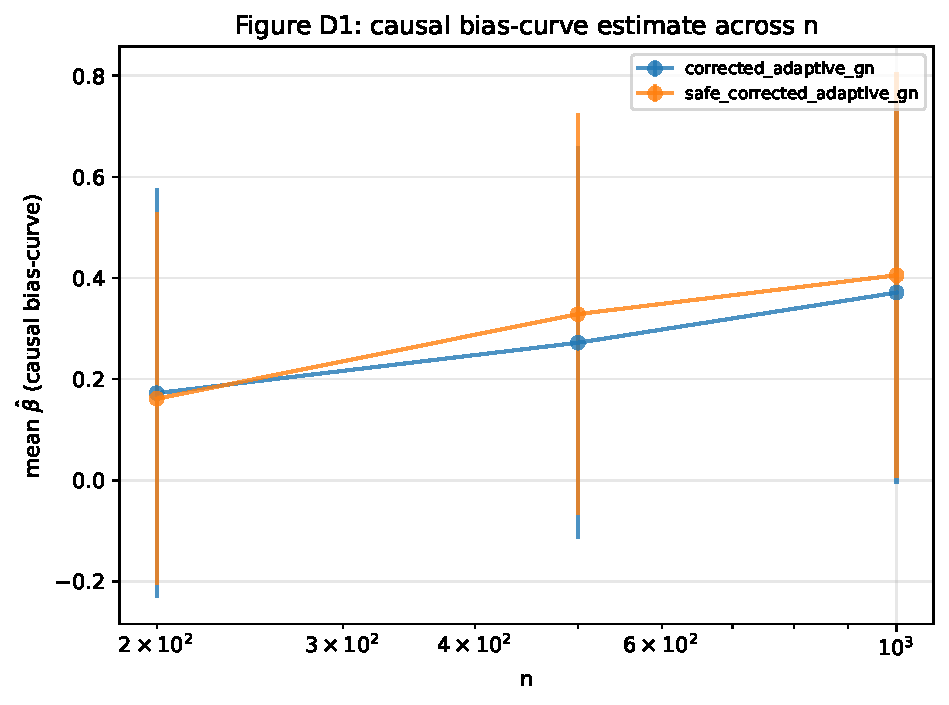
\includegraphics[width=\linewidth]{figures/figD1_causal_learning.pdf}
    \caption{ATE bias learning.}
    \label{fig:causal_learning}
  \end{subfigure}\hfill
  \begin{subfigure}[t]{0.48\linewidth}
    \centering
    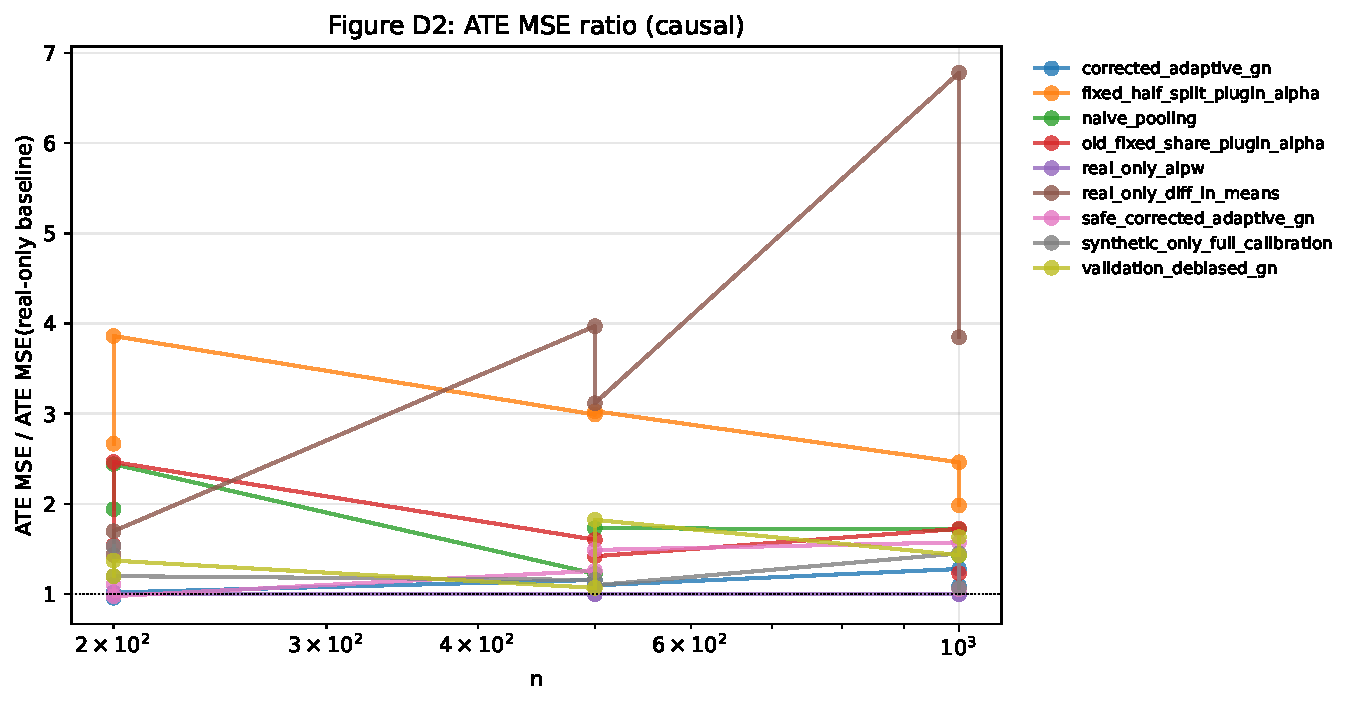
\includegraphics[width=\linewidth]{figures/figD2_ate_mse.pdf}
    \caption{ATE MSE ratios.}
    \label{fig:causal_mse}
  \end{subfigure}
  \caption{\emph{Left:} ATE bias learning curve for the IHDP-style semi-synthetic causal benchmark with a linear outcome generator. \emph{Right:} ATE MSE ratio to real-only AIPW. In this full-profile setting, the corrected adaptive method is mildly harmful in all 8 cells but avoids the much larger losses of the naive baselines.}
\end{figure}

% POLISHED
